\documentclass[border=8pt]{standalone}
\usepackage[T1]{fontenc}\usepackage[utf8]{inputenc}\usepackage{lmodern}
\usepackage{tikz}\usetikzlibrary{arrows.meta,positioning}
\begin{document}
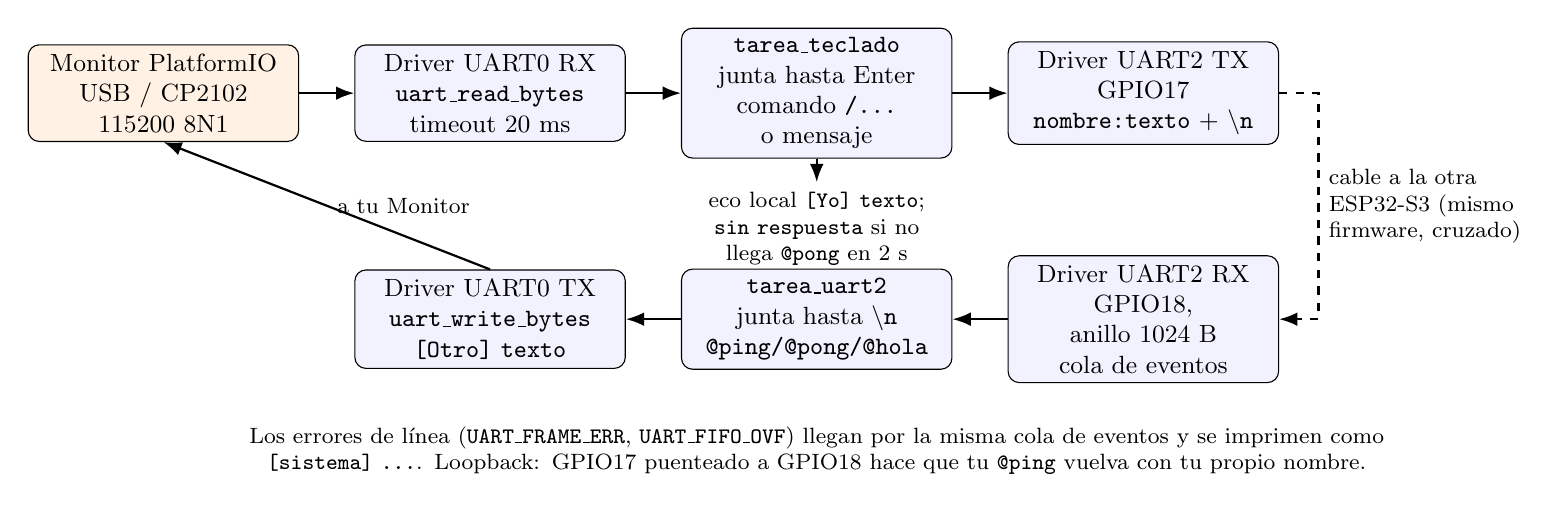
\begin{tikzpicture}[>=Latex,font=\small,node distance=0.7cm,
 b/.style={draw,rounded corners,fill=blue!5,text width=3.2cm,align=center,minimum height=1cm},
 h/.style={draw,rounded corners,fill=orange!10,text width=3.2cm,align=center,minimum height=1cm}]
% Ida: teclado del alumno -> UART0 -> tarea_teclado -> UART2 TX
\node[h] (mon) {Monitor PlatformIO\\USB / CP2102\\115200 8N1};
\node[b,right=of mon] (u0rx) {Driver UART0 RX\\\texttt{uart\_read\_bytes}\\timeout 20 ms};
\node[b,right=of u0rx] (tk) {\texttt{tarea\_teclado}\\junta hasta Enter\\comando \texttt{/...} o mensaje};
\node[b,right=of tk] (u2tx) {Driver UART2 TX\\GPIO17\\\texttt{nombre:texto} + \texttt{\textbackslash n}};
% Vuelta: UART2 RX -> cola de eventos -> tarea_uart2 -> UART0 TX
\node[b,below=1.4cm of u2tx] (u2rx) {Driver UART2 RX\\GPIO18, anillo 1024 B\\cola de eventos};
\node[b,left=of u2rx] (tu) {\texttt{tarea\_uart2}\\junta hasta \texttt{\textbackslash n}\\\texttt{@ping/@pong/@hola}};
\node[b,left=of tu] (u0tx) {Driver UART0 TX\\\texttt{uart\_write\_bytes}\\\texttt{[Otro] texto}};
\draw[->,thick] (mon)--(u0rx);\draw[->,thick] (u0rx)--(tk);\draw[->,thick] (tk)--(u2tx);
\draw[->,thick] (u2rx)--(tu);\draw[->,thick] (tu)--(u0tx);
\draw[->,thick] (u0tx.north) -- node[right,font=\footnotesize,align=left]{a tu Monitor} (mon.south);
\draw[->,thick,dashed] (u2tx.east) -- ++(0.5,0) |- node[pos=0.25,right,font=\footnotesize,align=left]{cable a la otra\\ESP32-S3 (mismo\\firmware, cruzado)} (u2rx.east);
\draw[->,thick] (tk.south) -- ++(0,-0.3) node[below,font=\footnotesize,text width=3.4cm,align=center]{eco local \texttt{[Yo] texto};\\\texttt{sin respuesta} si no llega \texttt{@pong} en 2 s};
\node[font=\footnotesize,text width=15cm,align=center,below=0.6cm of tu.south] {Los errores de línea (\texttt{UART\_FRAME\_ERR}, \texttt{UART\_FIFO\_OVF}) llegan por la misma cola de eventos y se imprimen como \texttt{[sistema] ...}. Loopback: GPIO17 puenteado a GPIO18 hace que tu \texttt{@ping} vuelva con tu propio nombre.};
\end{tikzpicture}
\end{document}
